\documentclass[12pt, twoside]{article}
% \documentclass[12pt, twoside]{article}
\usepackage[letterpaper, margin=1in, headsep=0.2in]{geometry}
\setlength{\headheight}{0.6in}
%\usepackage[english]{babel}
\usepackage[utf8]{inputenc}
\usepackage{microtype}
\usepackage{amsmath}
\usepackage{amssymb}
%\usepackage{amsfonts}
\usepackage[nomessages]{fp} %\FPeval{\var-name}{2*sin(pi/6)}
\usepackage{siunitx} %units in math. eg 20\milli\meter
\usepackage{yhmath} % for arcs, overparenth command
\usepackage{tikz} %graphics
\usetikzlibrary{quotes, angles, arrows, arrows.meta}
\usepackage{graphicx} %consider setting \graphicspath{{images/}}
\usepackage{parskip} %no paragraph indent
\usepackage{enumitem}
\usepackage{multicol}
\usepackage{venndiagram}

\usepackage{fancyhdr}
\pagestyle{fancy}
\fancyhf{}
\renewcommand{\headrulewidth}{0pt} % disable the underline of the header
\raggedbottom
\hfuzz=2mm %suppresses overfull box warnings

\usepackage{hyperref}
\usepackage{float}

\fancyhead[LE]{\thepage}
\fancyhead[RO]{\thepage \\ First and last name: \hspace{2.5cm} \,\\ Section: \hspace{2.5cm} \,}
\fancyhead[LO]{BECA / Dr. Huson / Regents Prep: Graphs\\* 2 December 2024}

\begin{document}

\subsubsection*{1.14 Do Now: Graphing inequalities}
\begin{enumerate}
  \item Graph and label the two inequalities on the grid. 

  \begin{multicols}{2}
    $\displaystyle y \geq 2x-2$ \\
    $x+ \frac{1}{2}y < 3$
    \end{multicols} \vspace{1cm}

  \begin{center} %4 quadrant regents grid w T-Chart
  \begin{tikzpicture}[scale=.635]
    \draw [help lines] (-10,-10) grid (10,10);
    \draw [thick, ->] (-10.2,0) -- (10.4,0) node [below right] {$x$};
    \draw [thick, ->] (0,-10.2)--(0,10.4) node [left] {$y$};
  \end{tikzpicture}
  \end{center}

Mark a point in the solution set and label it with the ordered pair.

\newpage
\item Which of the following would map $\triangle CAT \rightarrow \triangle C'A'T'$?  \vspace{0.5cm}
  \begin{multicols}{2}
    \begin{itemize}
      \item[T \quad F \quad] Reflected across the $y$-axis
      \item[T \quad F \quad] Translated six to the left, down zero
      \item[T \quad F \quad] Reflected across the $y$-axis, then slid to the left two
      \item[T \quad F \quad] $(x,y) \rightarrow (x-6, y+0)$
      %\item[T \quad F \quad] Rotated $90^\circ$ counterclockwise around the origin
      \item[T \quad F \quad] Reflected across the line $x=-1$
    \end{itemize}
    \begin{tikzpicture}[scale=.48]
      \draw [help lines] (-7,-4) grid (6,5);
      \draw [thick, <->] (-7.4,0) -- (6.4,0) node [right] {$x$};
      \draw [thick, <->] (0,-4.4)--(0,5.4) node [above] {$y$};  
      \draw [thick]
      (2,2) node[above] {$C$}--
      (4,1) node[right] {$A$}--
      (2,-2) node[below left] {$T$}--cycle;
      \draw [thick]
      (-4,2) node[above] {$C'$}--
      (-6,1) node[left] {$A'$}--
      (-4,-2) node[below left] {$T'$}--cycle;
    \end{tikzpicture}
  \end{multicols}

\item Draw the line of reflection for quadrilaterals in the diagram below.
  \begin{center}
  \begin{tikzpicture}[scale=.48]
    %\draw [help lines] (-10,-7) grid (10,7);
    \draw [thick, <->] (-4.4,0) -- (8.4,0) node [right] {$x$};
    \draw [thick, <->] (0,-2.4)--(0,7.4) node [above] {$y$};  
    \draw [thick](5,1)--(6,4)--(8,5)--(4,5)--cycle;  
    \draw [thick](-1,1)--(-2,4)--(-4,5)--(0,5)--cycle;
  \end{tikzpicture}
\end{center}

\item The quadrilateral $ROCK$ undergoes rigid motions, shown below. Describe the sequence of transformations applied.
  \begin{flushright}
      \begin{tikzpicture}[scale=.48]
      \draw [help lines] (-6,-7) grid (10,5);
      \draw [thick, <->] (-6.4,0) -- (10.4,0) node [right] {$x$};
      \draw [thick, <->] (0,-7.4)--(0,5.4) node [above] {$y$};  
      \draw [thick]
        (5,1) node[below] {$K''$}--
        (5,3) node[above left] {$R''$}--
        (7,4) node[right] {$O''$}--
        (8,1) node[right] {$C''$}--cycle;
      \draw [thick]
        (-2,1) node[below] {$K'$}--
        (-2,3) node[above left] {$R'$}--
        (0,4) node[right] {$O'$}--
        (1,1) node[right] {$C'$}--cycle;  
      \draw [thick]
      (-2,-3) node[left] {$K$}--
      (-2,-5) node[left] {$R$}--
      (0,-6) node[right] {$O$}--
      (1,-3) node[right] {$C$}--cycle;
    \end{tikzpicture}
  \end{flushright}


\end{enumerate}
\end{document}